\documentclass{article}
\usepackage{amsmath}
\usepackage{amssymb}
\usepackage[fontsize=16pt]{fontsize}
\usepackage{setspace}
\usepackage{graphicx}
\usepackage[skip=10pt plus1pt, indent=10pt]{parskip}
\usepackage{tikz}

\author{}
\date{}
\title{\textbf{Radicals \& Surds Course}\\
\vspace{28pt}
\begin{center}

\includegraphics[width=4em]{ApS_logo.png}
\end{center}
\begin{normalsize}
Applied Scholastics, Ferndale WA
\end{normalsize}}

\begin{document}
\maketitle

\setstretch{1.2}

\section*{Radicals}

Radical is Latin for root. In conversation it means a complete or drastic change, as if going all the way to the roots of a problem. "A radical new idea," for example. In maths it means the roots of a number and it is the name of the $\sqrt$ symbol that is used for writing roots of numbers. $\sqrt{25}$ is a radical.

The value in the radical symbol is known as the radicand.

The small number to the left of the radical symbol is called the order of the radical. It is also known as the index. The order of a root indicates which root you are taking. It is how many times you need to multiply a number by itself to get the radicand.

\begin{enumerate}

\item What does radical mean, in everyday speech?
\item Use radical in a sentence, with that meaning.
\item What does radical mean in maths?
\item Use radical in a sentence, with that meaning.
\item What is the radical sign?
\item Give an example of a radical expression.
\item What is a radicand?
\item Use radicand in a sentence.
\item What is the order of a root?
\item What is the order of $\sqrt[4]{16}$?

\section*{Surds}

\subsection*{Rational and Irrational Numbers}

A rational number is a number that can be written as a ratio of two whole numbers.

$1, \frac{2}{3}, -4, \frac{273}{8}$ are all rational numbers.

Numbers that can’t be written as the ratio of two whole numbers are called irrational numbers.

For example, the ratio between the circumference of a circle and its diameter, known by the Greek letter $\pi$ (pi), which stands for ‘perimeter,’ cannot be written exactly as a ratio of any two whole numbers so it is called an irrational number.

\item What does rational mean?
\item What is a rational number?
\item What do ratios have to do with rational numbers?
\item Give an example of a rational number.
\item Give an example of an irrational number.

\subsection*{Surds}

‘Surd’ is a Latin word meaning ‘deaf, mute.’ Surds are irrational numbers that can only be written as the root of an integer because they are not a rational number. They cannot be simplified further.

$\sqrt{9}$ is not a surd because $\sqrt{9}=3$ exactly.

$\sqrt{2}$ is a surd because $\sqrt{2}\approx 1.41421\ldots$ and can only be written exactly as $\sqrt{2}$.

A surd with a single term, such as $\sqrt{7}$ or $\sqrt{2}$ is called a simple surd or a monomial surd.

A surd with two terms, such as $\sqrt{7}-\sqrt{2}$ or $x\sqrt[4]{a}-b$ is called a binomial surd or a compound surd.

Usually surds are left as they are in expressions so that an accurate answer can be reached, and only at the final step is a decimal approximation given if needed.

\item What is a surd?
\item Why are they called surds?
\item Use surd in a sentence.
\item Give an example of a simple surd.
\item Give an example of a compound surd.
\item Is $\pi$ a surd?
\item Are all irrational numbers surds?

\subsection*{Some famous surds}

There are many instances of surds that arise in geometry and in other areas of maths.

\subsubsection*{Pythagoras}

Pythagoras was a famous Greek mathematician who lived in the fifth century BC.

A right angle means an angle of $90^{\circ}$, like the angle between a flat floor and an upright wall.

A right triangle is one that has one right angle.

In a right triangle, the longest side is called the hypotenuse, which is Greek for "stretch under." The hypotenuse is always opposite to the right angle and could be said to stretch under it.

\item Who was Pythagoras?
\item What is a right angle?
\item What is a right triangle?
\item What is a hypotenuse?

A theorem is a proven statement of a mathematical truth. 

\item What is a theorem?
\item Use theorem in a sentence.

\begin{tikzpicture}
  \coordinate (A) at (0,0);
  \coordinate (B) at (5,0);
  \coordinate (C) at (0,3);
  \draw (A) -- (B) -- (C) -- cycle;
  \node at (2.5,-0.3) {$a$};
  \node at (-0.3,1.5) {$b$};
  \node at (2.8,1.8) {$c$};
  \draw (A) -- (-3,0) -- (-3,3) -- (C);
  \draw (A) -- (0,-5) -- (5,-5) -- (B);
  \draw (B) -- (8,5) -- (3,8) -- (C);
  \draw (0,0.6) -- (0.6,0.6) -- (0.6,0)
  \node at (0.3,0.3) {\tiny{$90^{\circ}$}};
  \node at (-1.5,1.5) {$b^2$};
  \node at (2.5,-2.5) {$a^2$};
  \node at (4,4) {$c^2$};
  \node at (3,-6) {Pythagoras' Theorem: $c=\sqrt{a^2+b^2}$}
\end{tikzpicture}

Pythagoras' most famous theorem states that the length of the hypotenuse of a right triangle is the square root of the sum of the squares of the other two sides. In other words, for a right triangle with sides of length a, b and c, where c is the hypotenuse, $c^2=a^2+b^2$, so $c=\sqrt{a^2+b^2}$. This radical expression is very well known and useful.

\item What is Pythagoras' Theorem?
\item What does Pythagoras' Theorem have to do with radicals and surds?

\subsubsection*{Theodorus}

Theodorus was another Greek mathematician from the fifth century BC.

Theodorus is known for the "spiral of Theodorus" which is built of right triangles. The hypotenuse lengths, following Pythagoras' Theorem, are the square root of each integer in turn, many of which are surds.

\begin{center}
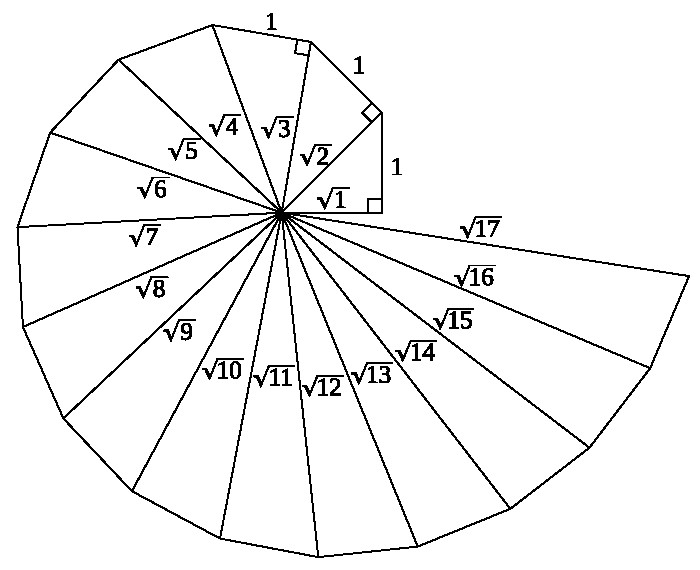
\includegraphics[width=\linewidth]{Spiral_of_Theodorus.jpg}
\caption{The spiral of Theodorus}
\end{center}

\item What is the spiral of Theodosus?
\item What does the spiral of Theodorus have to do with radicals and surds?
\item The spiral of Theodorus fits the the square roots of integers 1 to 17 before it starts to overlap on itself. Which of these lengths are surds?

\subsubsection*{The Golden Ratio}

The golden ratio, denoted by the Greek letter $\phi$ (phi), is a mathematical constant, a surd, that is found in many places in nature. It has fascinated mathematicians, artists, and architects for centuries.

$$\phi=\frac{1+\sqrt{5}}{2}\approx1.61803398875$$

$\phi$ can be derived from line segments that follow this golden ratio, such that the ratio of the length of two line segments to their total length is equal to the ratio of their lengths.

\begin{center}
\begin{tikzpicture}
\draw (0,0) -- (7,0);
\draw (0,0.2) -- (0,-0.2);
\draw (4.5,0.2) -- (4.5,-0.2);
\draw (7,0.2) -- (7,-0.2);
\node at (2.2,0.5) {$a$};
\node at (5.7,0.5) {$b$};
\end{tikzpicture}
\end{center}

$$\frac{a+b}{a}=\frac{a}{b}$$

Which resolves to give $\phi=\frac{1+\sqrt{5}}{2}.$

$\phi$ can also be expressed as a continued fraction:

\begin{equation*}
\phi = 1 + \cfrac{1}{1 + \cfrac{1}{1 + \cfrac{1}{1 + \ldots}}}
\end{equation*}

And $\phi$ can be derived from sectioning a rectangle in a way that creates a similar rectangle. Consider a rectangle with sides $a$ and $b$.

Create a square inside a rectangle while maintaining the proportion between the original rectangle and the new one.

If we set the length of b to 1 then the smaller rectangle that is created must have sides of length $a-1$ and $1$.

\begin{center}
\begin{tikzpicture}
  \draw (0,0) -- (4.854,0) -- (4.854,3) -- (0,3) -- (0,0);
  \draw (3,0) -- (3,3);
  \draw (-0.15,1.4) -- (0.15,1.45)
  \draw (-0.15,1.3) -- (0.15,1.35)
  \draw (1.5,3.15) -- (1.45,2.85)
  \draw (1.6,3.15) -- (1.55,2.85)
  \node at (2.4,-0.5) {$a$};
  \node at (5.5,1.5) {$b$};
  \node at (3.8,3.5) {$a-1$};
  \node at (1.5,3.5) {1}
  \node at (-0.5,1.5) {1}
\end{tikzpicture}
\end{center}

The smaller rectangle, with sides of lengths $(a-1)$ and $1$, is in proportion to the original rectangle, with sides of lengths $1$ and $a$, so we can say that $\frac{1}{a}=\frac{a-1}{1}$, which again can be solved to give $\phi=\frac{1+\sqrt{5}}{2}$.

The rectangle can in fact be divided infinitely in this way, creating a spiral, with rectangles all in the same ratio.

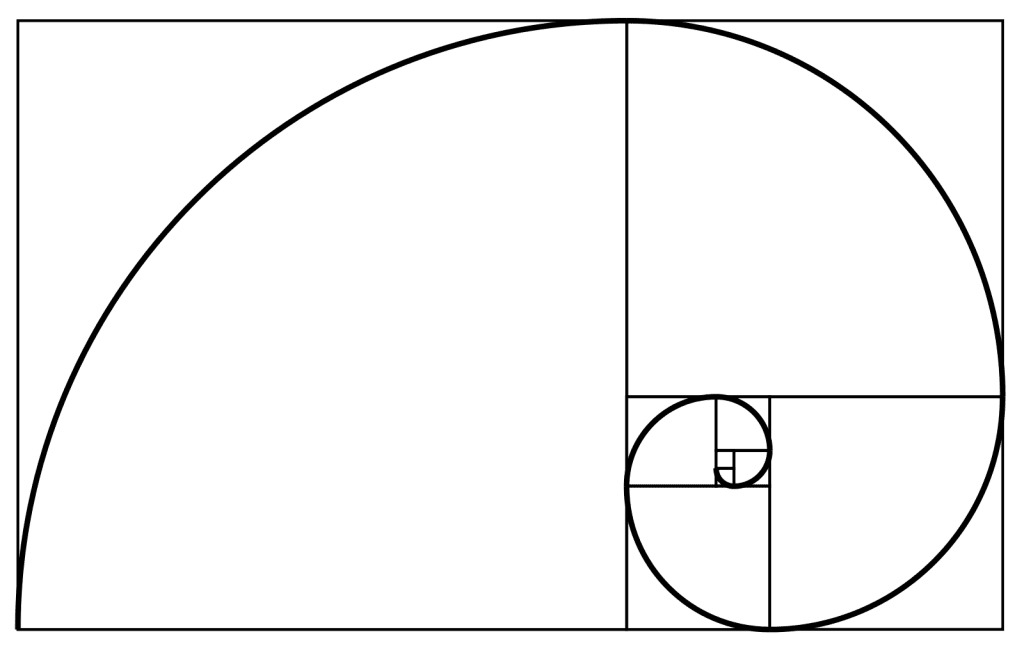
\includegraphics[width=\textwidth]{Ratio-1024x648.png}

\section*{Surd Laws}

\setstretch{1.2}
The laws of radicals and surds are derived from the Power Laws. (Remember that radicals and surds are equivalent to fractional powers.)

\subsection*{Multiplication and Division\\ of Surds}
\begin{align*}
\sqrt{a} \cdot \sqrt{b}&=\sqrt{ab}\\
\frac{\sqrt{a}}{\sqrt{b}}&=\sqrt{\frac{a}{b}}\\
(\sqrt[n]{a})^n&=a
\end{align*}
$$\text{e.g. }\sqrt{32}\times\sqrt{2}=\sqrt{32\times2}=\sqrt{64}=8.$$
$$\text{e.g. }\sqrt{12}\div\sqrt{3}=\sqrt{12\div3}=\sqrt{4}=2.$$
$$\text{e.g. }(\sqrt[3]{5})^3=5$$

\item Calculate $\frac{\sqrt[3]{81}}{\sqrt[3]{9}}$
\item Calculate $\sqrt{48}\div\sqrt{12}$
\item Calculate $\sqrt{50}\cdot\sqrt{2}$
\item Calculate $(\sqrt{6} + \sqrt{3})(\sqrt{6})$
\item Calculate $\frac{2\sqrt{5}}{\sqrt{5} - \sqrt{2}}$
\item Calculate $(\sqrt{2} - \sqrt{3})(\sqrt{2})$
\item Calculate $\frac{\sqrt{5} - \sqrt{7}}{\sqrt{3} + \sqrt{5}}$
\item Calculate $\frac{2\sqrt{6}}{\sqrt{3} - \sqrt{2}}$

\subsection*{Simplification of Surds}

Surd is sometimes used as a synonym for radical, but surds and radicals are actually different things. In the same way that all composite numbers can be broken down and expressed as a product of prime numbers, all radicals can be broken down and expressed as the product of whole numbers and radicals.

Surds are easier to understand and handle in their simplified form. The chance of mistakes is lessened, and because they are put into a standardized form, it is easier to see what mathematical rules apply.

To simplify a surd expression, list the factors of the radicand, choose two of them, one of which must be a square number, and then use the rule $\sqrt{mn}=\sqrt{m}\sqrt{n}$.

For larger numbers, first list out the prime factors of the radicand and then spot matching pairs.

e.g. $\sqrt{24}$:
\begin{center}
\begin{tikzpicture}
  [level distance=1cm,
  level 1/.style={sibling distance=2cm},
  level 2/.style={sibling distance=2cm}]
  \node {24}
    child {node {2}}
    child {node {12}
      child {node {2}}
      child {node {6}
        child {node {2}}
        child {node {3}}}};
\end{tikzpicture}\\
$24=$\underline{$2\times2$}$\times2\times3$
\end{center}
\begin{align*}
\sqrt{24}&=\sqrt{(2\times2)\times2\times3}\\
&=\sqrt{2\times2}\times\sqrt{2\times3}\\
&=4\sqrt{6}
\end{align*}
\begin{align*}
\text{e.g. }
\sqrt{50}&=\sqrt{2\times25}\\
&=\sqrt{2}\times\sqrt{25}\\
&=\sqrt{2}\times5=5\sqrt{2}\\
\end{align*}
\begin{align*}
\text{e.g. }
\sqrt{18}
&=\sqrt{2 \times 9}\\
&=\sqrt{2} \times \sqrt{9}\\
&=\sqrt{2} \times 3=3\sqrt{2}\\
\end{align*}
\begin{align*}
\text{e.g. }
\sqrt{147}-2\sqrt{12}
&=\sqrt{49 \cdot 3}-2\sqrt{4 \cdot 3}\\
&=\sqrt{49} \cdot \sqrt{3}-2\sqrt{4} \cdot \sqrt{3}\\
&=7\sqrt{3}-2 \cdot 2\sqrt{3}\\
&=7\sqrt{3}-4\sqrt{3}\\
&=3\sqrt{3}
\end{align*}

\item What is the purpose of simplifying expressions that contain radicals and surds?
\item What is the procedure for simplifying expressions that contain radicals and surds?
\item Simplify $\sqrt{48}$
\item Simplify $\sqrt{60}$
\item Simplify $\sqrt{20}$
\item Simplify $\sqrt{2}\cdot\sqrt{2}$
\item Simplify $\sqrt{50}\cdot\sqrt{2}$
\item Simplify $\sqrt{48}\div\sqrt{12}$
\item Simplify $\sqrt[3]{81}\cdot\sqrt[3]{9}$
\item Simplify $\sqrt[4]{128}\cdot\sqrt[4]{2}$
\item Simplify $4\sqrt{2}-\sqrt{5}+\sqrt{3}-2(\sqrt{5}-\sqrt{2})$
\item Simplify $\sqrt{50}+\sqrt{8}-\sqrt{48}$

\subsection*{Comparing Surds}

\subsubsection*{comparing surds of the same order}
Surds of the same order can be compared by simply comparing the radicands.

$$\sqrt{5}<\sqrt{6}<\sqrt{7}$$
$$\sqrt[4]{2}<\sqrt[4]{3}<\sqrt[4]{4}$$

\item How do you compare surds of the same order?
\item Compare $\sqrt{15}$ and $\sqrt{20}$.

\subsubsection*{comparing surds of different orders}
Surds of different orders, before they can be compared, have to be converted to the lowest common multiple of their orders.

You can change the order of a radical by multiplying the order and the radicand by the same amount.

e.g. Compare $\sqrt{3$}, $\sqrt[3]{2}$ and $\sqrt[4]{4}$\ :
\begin{align*}
\sqrt[2]{3}&=\sqrt[2\times6]{3\times6}=\sqrt[12]{18}\\
\sqrt[3]{2}&=\sqrt[3\times4]{2\times6}=\sqrt[12]{12}\\
\sqrt[4]{4}&=\sqrt[4\times3]{4\times6}=\sqrt[12]{24}\\
\text{Thus }\sqrt[3]{2}&<\sqrt{3}<\sqrt[4]{4}
\end{align*}

\item How do you compare surds of diffrerent orders?
\item Compare $\sqrt[3]{15}$ and $\sqrt[4]{20}$.

\subsubsection*{comparing multiples of surds}
To compare multiples of surds it may be necessary to reverse the simplification so each surd is expressed as a single radical instead of as surds with coefficients.

e.g. Comparing $2\sqrt{5}$ and $5\sqrt{2}$ :
\begin{align*}
2\sqrt{5}&=\sqrt{2}\sqrt{2}\sqrt{5}=\sqrt{2\times2\times5}=\sqrt{20}\\
5\sqrt{2}&=\sqrt{5}\sqrt{5}\sqrt{2}=\sqrt{5\times{5\times{2}}}=\sqrt{50}\\
&\text{Thus }2\sqrt{5}<5\sqrt{2}
\end{align*}

\item How do you compare multiples of surds?
\item Compare $3\sqrt{5}$ and $2\sqrt{10}$.

\subsection*{Like Surds}

\paragraph{Coefficients}
A coefficient is the number that goes before and multiplies another quantity in algebra. In "$5x$" or "$5\sqrt{3}$", the "5" is the coefficient.

\item What is a coefficient?
\item Write 5 examples of coefficients.

Radicals can be reduced to their simplest form as a product of coefficients and surds.

Surds that are of the same order and that have the same radicand, or unsimplified multiples of these, are called "like surds." You can only add or subtract like surds.

You cannot directly add or subtract surds with different roots or different radicands.

$$\text{e.g. }\sqrt{2}+\sqrt{2}=2\sqrt{2}$$
$$\text{e.g. }3\sqrt[3]{5}-\sqrt[3]{5}=2\sqrt[3]{5}$$
$$\text{e.g. }\sqrt{12}+\sqrt{48}=2\sqrt{3}+4\sqrt{3}=6\sqrt{3}$$
\item What are like surds?
\item Can you add and subtract surds that are not like surds?
\item What is $\sqrt{20}+\sqrt{80}$?
\item What is $\sqrt[3]{64}-\sqrt[4]{256}$?
\item What is $\sqrt{18}-\sqrt{72}$?
\item What is $\sqrt[3]{32}+\sqrt{200}$?
\item What is $\sqrt[3]{64}-\sqrt[4]{256}$?
\item What is $\sqrt[4]{32}+\sqrt[4]{128}$?

\subsection*{Rationalizing the Denominator}

Rationalizing, in maths, means expressing something as a ratio, such as a fraction. The denominator means the number on the bottom of a fraction which says what sort of fraction it is. So rationalizing the denominator means getting rid of the irrational surd on the bottom of a fraction.

That makes it easier to calculate a decimal number value for a surd, and it is easier generally to have the surds in the numerator rather than in the denominator of expressions.

Without a calculator, working out $\frac{3}{\sqrt{2}}$ requires the tedious long division of $3\div1.4142\ldots}$.

To rationalize $\frac{a}{\sqrt{b}}$, multiply by $\frac{\sqrt{b}}{\sqrt{b}}$\ :

$$\frac{3}{\sqrt{2}}\cdot
\frac{\sqrt{2}}{\sqrt{2}}
=\frac{3\sqrt{2}}{2}\\
\approx2.1213$$

\begin{align*}
\text{e.g. }
\frac{1}{\sqrt{3}}
&=\frac{1}{\sqrt{3}}\cdot \frac{\sqrt{3}}{\sqrt{3}}\\
&=\frac{1\sqrt{3}}{\sqrt{3}\sqrt{3}}=\frac{\sqrt{3}}{3}
\end{align*}

\begin{align*}
\text{e.g. }
\frac{\sqrt{3}}{\sqrt{2}}+\frac{2}{\sqrt{6}}
&=\frac{\sqrt{3}}{\sqrt{2}}\cdot
\frac{\sqrt{3}}{\sqrt{3}}
+\frac{2}{\sqrt{6}}\\
&=\frac{3}{\sqrt{6}}+\frac{2}{\sqrt{6}}
=\frac{5}{\sqrt{6}}\\
&=\frac{5}{\sqrt{6}}\cdot\frac{\sqrt{6}}{\sqrt{6}}\\
&=\frac{5\sqrt{6}}{6}
\end{align*}

\item Rationalize the denominator of $\frac{1}{\sqrt{5}}$.
\item Rationalize the denominator of $\frac{1}{\sqrt{8}}$.
\item Rationalize the denominator of $\frac{1}{\sqrt{2}+1}$.
\item Rationalize the denominator of $\frac{3}{\sqrt{7}}$.
\item Rationalize the denominator of $\frac{5}{\sqrt{3}+\sqrt{2}}$.

\subsubsection*{Using Difference of Squares}

\paragraph{Quadratics}
Quadratic means ‘to do with a square’ and is from the Latin word quad, for four.

A quadratic equation has one or more square terms, such as $x^2+1=5$.

A quadratic surd is a surd, or an expression containing a surd, that has an index of 2. They are 'square roots’ such as $\sqrt{2}$, $\sqrt{5}$, or $3\sqrt{10}$.

\item What does quadratic mean?
\item What is a quadratic equation?
\item Give an example of a quadratic equation.
\item What is a quadratic surd?
\item Give an example of a quadratic surd.

\paragraph{Conjugates}
A conjugate is a pair of joined or related opposites, such as the sum and difference $(a+b)(a-b)$. Conjugates have various applications in mathematics, including simplifying expressions and solving equations. Conjugates of quadratic surds are useful because they multiply to produce a rational number.

\item What is a conjugate?
\item Use conjugate in a sentence.
\item Why are conjugates useful?

\paragraph{Difference of Squares Formula}
The difference of squares formula is that the product of the sum and difference of two values is equal to the difference of their squares:

$$(a+b)(a-b)=a^2-b^2.$$

\paragraph{Conjugate Surds}
The denominator of a quadratic surd can be rationalized using the difference of squares formula by making conjugate surd pairs.

The sum and difference of $n\sqrt{a}$ and $n\sqrt{b}$ are $(n\sqrt{a}+m\sqrt{b})$ and $(n\sqrt{a}-m\sqrt{b})$.

\begin{align*}
\text{e.g. }(3+\sqrt{2})(3-\sqrt{2})
&=3^2-{\sqrt{2}}^2\\
&=9-2=7\\\\
\textrm{e.g. }(\sqrt{2}+\sqrt{3})(\sqrt{2}-\sqrt{3})
&={\sqrt{2}}^2-{\sqrt{3} }^2\\
&=2-3=-1
\end{align*}

To rationalize \large$\frac{a}{b+\sqrt{c}}$\normalsize, multiply the numerator and denominator by the conjugate of the denominator, $b-\sqrt{c}$.
$$\frac{a}{b+\sqrt{c}}=\frac{a}{b+\sqrt{c}}\\\cdot\frac{b-\sqrt{c}}{b-\sqrt{c}}$$
To rationalize \large$\frac{a}{b-\sqrt{c}}$\normalsize, multiply the numerator and denominator by the conjugate of the denominator, $b+\sqrt{c}$.
$$\frac{a}{b-\sqrt{c}}=\frac{a}{b-\sqrt{c}}\\\cdot\frac{b+\sqrt{c}}{b+\sqrt{c}}$$

\begin{equation*}
\begin{split}
\textrm{e.g. }
\frac{1}{\sqrt{7}+\sqrt{5}}
&=\frac{1}{\sqrt{7}+\sqrt{5}}
\cdot\frac{\sqrt{7}-\sqrt{5}}{\sqrt{7}-\sqrt{5}}\\
&=\frac{\sqrt{7}-\sqrt{5}}{(\sqrt{7})^2-(\sqrt{5})^2}\\
&=\frac{\sqrt{7}-\sqrt{5}}{7-5}\\
&=\frac{\sqrt{7}-\sqrt{5}}{-2}
\end{split}
\end{equation*}

\begin{align*}
\text{e.g. }
\frac{3}{2+\sqrt{5}}
&=\frac{3}{2+\sqrt5}\cdot\frac{2-\sqrt{5}}{2-\sqrt{5}}\\
&=\frac{3(2-\sqrt{5})}{(2+\sqrt{5})(2-\sqrt{5})}\\
&=\frac{6-3\sqrt{5}}{4+2\sqrt{5}-2\sqrt{5}-5}\\
&=\frac{6-3\sqrt{5}}{-1}\\
&=3\sqrt{5}-6
\end{align*}

\begin{align*}
\text{e.g. }
\frac{\sqrt{3}+\sqrt{2}}
{3\sqrt{2}+2\sqrt{3}}
&=\frac{\sqrt{3}+\sqrt{2}}
{3\sqrt{2}+2\sqrt{3}}\cdot
\frac{3\sqrt{2}-2\sqrt{3}}
{3\sqrt{2}-2\sqrt{3}}\\
&=\frac{3\sqrt{2}\sqrt{3}
-2{\sqrt{3}}^2
+3{\sqrt{2}}^2
-2{\sqrt{3}}^2}
{(3\sqrt{2})^2-(2\sqrt{3})^2}\\
&=\frac{2\sqrt{3}-2{\sqrt{3}}^2+3{\sqrt{2}}^2}
{3^2{\sqrt{2}}^2-2^2{\sqrt{3}}^2}\\
&=\frac{\sqrt{6}-(2\cdot3)+(3\cdot2)}{(9\cdot2)-(4\cdot3)}\\
&=\frac{\sqrt{6}}{6}
\end{align*}

\item Rationalize the denominator of $\frac{2}{3 + \sqrt{5}}$
\item Rationalize the denominator of $\frac{5}{1 + \sqrt{3}}$
\item Rationalize the denominator of $\frac{3}{2 + \sqrt{8}}$
\item Rationalize the denominator of $\frac{4}{5 + \sqrt{20}}$
\item Rationalize the denominator of $\frac{7}{6 + \sqrt{18}}$
\item Rationalize the denominator of $\frac{\sqrt{2} - \sqrt{3}}{\sqrt{5} + \sqrt{7}}$

\end{enumerate}

\end{document}
